\documentclass[10pt]{article}
\usepackage[margin=0.65in]{geometry}
\usepackage{graphicx,booktabs,array,xcolor,hyperref}
\usepackage[T1]{fontenc}
\usepackage[utf8]{inputenc}
\hypersetup{colorlinks=true,linkcolor=blue,urlcolor=blue}
\setlength{\parindent}{0pt}
\setlength{\parskip}{5pt}
\newcommand{\gae}{\mathrm{GAE}}
\begin{document}
\begin{center}
{\LARGE Independent factor-base / graph replication}\\[3pt]
{\small Run \texttt{20261024T2258Z-factor-base-replication} · protocol \texttt{factor-base-graph-replication/20261024/v1}}
\end{center}

The frozen five-arm protocol ran on a second cohort of 1,260 public
known-answer targets. The producer recorded 6,300 candidate solves and 6,300
paired source-negation-rho solves. Every answer was checked by recomputing the
scalar multiple on the source curve. Target scalars and algorithm seeds use
separate SHA-256 domains. The validator found zero seed, scalar, or target-point
overlaps with the original cohort.

\begin{center}
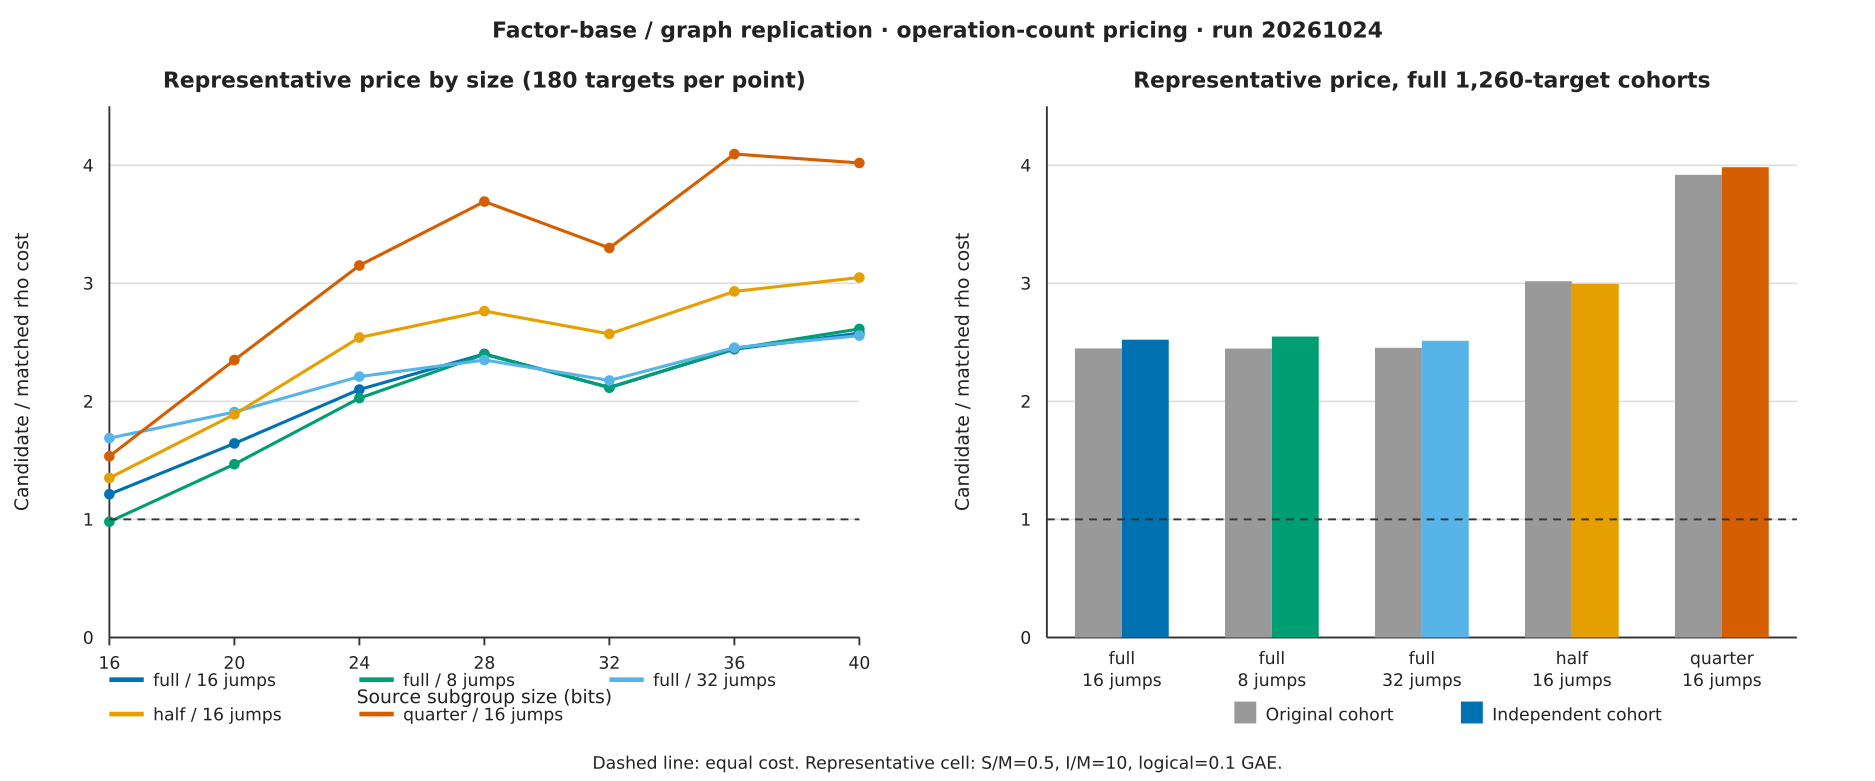
\includegraphics[width=\textwidth]{factor-base-replication.png}
\end{center}

\section*{Full-cohort operation counts and prices}
The representative cell is $S/M=0.5$, $I/M=10$, and 0.1 source-addition
equivalents per logical operation. Costs are sums over 1,260 targets. The band
is the minimum and maximum aggregate ratio over all 36 cells.

\small
\begin{tabular}{@{}lrrrrr@{}}
\toprule
Arm & Candidate $\gae$ & Rho $\gae$ & Ratio & 36-cell band & W/L/T \\
\midrule
Full, 16 jumps & 2,661,363,462 & 1,054,951,912 & 2.522734 & 1.386374--13.514033 & 0/36/0 \\
Full, 32 jumps & 2,651,510,986 & 1,054,951,912 & 2.513395 & 1.383840--13.440233 & 0/36/0 \\
Full, 8 jumps & 2,689,869,404 & 1,054,951,912 & 2.549755 & 1.401397--13.639329 & 0/36/0 \\
Half, 16 jumps & 3,159,731,682 & 1,054,951,912 & 2.995143 & 1.715544--16.504039 & 0/36/0 \\
Quarter, 16 jumps & 4,203,242,635 & 1,054,951,912 & 3.984298 & 2.388390--22.870499 & 0/36/0 \\
\bottomrule
\end{tabular}
\normalsize

One size-only slice has mixed results: full base with eight jumps at 16 bits
has 23 winning and 13 losing cells, representative ratio 0.980993, and band
0.790906--2.450390. Every other arm/size slice has zero winning cells.

\section*{Original and replication cohorts}
\small
\begin{tabular}{@{}lrrrrrr@{}}
\toprule
Arm & Original & Replication & Ratio delta & Old divisors & New divisors & Delta \\
\midrule
Full, 16 & 2.448830 & 2.522734 & +0.073904 & 219,581,773 & 219,259,871 & -321,902 \\
Full, 32 & 2.453278 & 2.513395 & +0.060117 & 219,864,588 & 218,282,418 & -1,582,170 \\
Full, 8 & 2.447173 & 2.549755 & +0.102582 & 220,092,171 & 221,972,970 & +1,880,799 \\
Half, 16 & 3.017732 & 2.995143 & -0.022589 & 282,983,105 & 272,004,613 & -10,978,492 \\
Quarter, 16 & 3.919193 & 3.984298 & +0.065105 & 392,583,830 & 387,233,280 & -5,350,550 \\
\bottomrule
\end{tabular}
\normalsize

These are two deterministic cohorts with one algorithm seed per target. No
sampling interval is assigned; the table records cohort differences without a
significance claim.

\section*{Validation and scope}
The independent native validator recomputed 6,300 target/seed derivations,
12,600 source scalar checks, 40 arm/slice summaries, and all 36 pricing cells
per summary. It reports \texttt{ok: true}. All 35 raw files have 180 records and
exit status 0.

\begin{tabular}{@{}p{0.38\textwidth}p{0.18\textwidth}p{0.36\textwidth}@{}}
\toprule
Requirement & Status & Evidence or limit \\
\midrule
Independent 1,260-target cohort & Verified complete & Zero seed/scalar/point overlaps \\
Five arms and paired rho & Verified complete & 6,300 candidate plus 6,300 rho records \\
All costs, wins, and losses & Verified complete & 1,440 aggregate price rows \\
Independent-host replay & Not attempted & No second-host receipt \\
Isolated wall / external-tool comparison & Not attempted & Counts only; elapsed times diagnostic \\
Leaderboard promotion & Not proposed & Replay and isolated wall gates absent \\
\bottomrule
\end{tabular}

The observations apply to the fixed public Scholten models, target derivation,
collector, rho implementation, and pricing contract. Machine-readable evidence,
checksums, and commands are documented in \texttt{DATA\_DICTIONARY.md} and
\texttt{results/manifest.json}.
\end{document}
